\documentclass[]{standalone}%
%
\usepackage{tikz}%
\usetikzlibrary{angles, arrows.meta, backgrounds, calc, decorations.pathmorphing, shapes.geometric, patterns, positioning}%
%
\definecolor{TUMBlack}{cmyk}{0,0,0,1}%
\definecolor{TUMBlue}{cmyk}{1,0.43,0,0}%           Pantone 300
\definecolor{TUMBlue1}{cmyk}{1,0.57,0.12,0.7}%     Pantone 540
\definecolor{TUMBlue2}{cmyk}{1,0.54,0.04,0.19}%    Pantone 301
\definecolor{TUMBlue3}{cmyk}{0.65,0.19,0.01,0.04}% Pantone 542
\definecolor{TUMBlue4}{cmyk}{0.42,0.09,0,0}%       Pantone 283
\definecolor{TUMOrange}{cmyk}{0,0.65,0.95,0}%
\definecolor{TUMGreen}{cmyk}{0.35,0,1,0.2}%
%
\begin{document}%
%
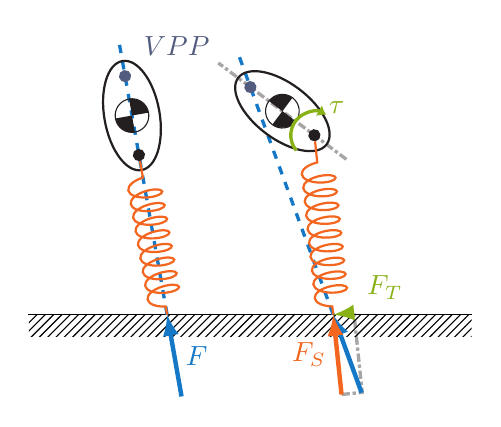
\begin{tikzpicture}[scale = 1]%
    %
    \def\groundheight{.8em}%
    \def\groundwidth{16em}%
    \def\comradius{.6em};%
    %
    \tikzstyle{arrow} = [->, -latex, ultra thick, draw = TUMBlack]%
    \tikzstyle{dashedline} = [draw = TUMBlue, dashed, very thick]%
    \tikzstyle{dot} = [circle, minimum size = .4em, inner sep = 0em, fill = TUMBlack, draw = TUMBlack]%
    \tikzstyle{com} = [circle, inner sep = .43em, draw = TUMBlack]%
    \tikzstyle{ground} = [fill = TUMBlack, pattern = north east lines, draw = none, minimum width = \groundwidth, minimum height = \groundheight]%
    \tikzstyle{spring} = [decoration = {coil, aspect = 0.4,  segment length = .5em,  amplitude = .6em,  pre length = .3em, post length = .3em}, decorate, thick, draw = TUMOrange]%
    \tikzstyle{oval} = [ellipse, minimum width = 2em, minimum height = 4em, draw = TUMBlack, solid, thick]%
    %
    \def\springmass(#1){% Syntax (center)
        \draw (#1) node [dot, draw = TUMBlue2!70!TUMOrange, fill = TUMBlue2!70!TUMOrange, transform shape] (v) {};%
        \draw (v) node [com, below = .6em of v, transform shape] (E) {};%
        \draw node [dot, below = .6em of E, transform shape] (t) {};%
        \node [oval, transform shape] () at (E) {};%
        \draw [spring] (A) -- (t);%
        %
        \clip (E) circle (\comradius);%
        \begin{scope}%
            \fill[TUMBlack] let \p1 = (E) in (\x1, \y1) (\x1 + \comradius, \y1) rectangle (\x1, \y1 + \comradius);%
            \fill[TUMBlack] let \p1 = (E) in (\x1, \y1) (\x1 - \comradius, \y1) rectangle (\x1, \y1 - \comradius);%
        \end{scope}%
    }
    %
    \def\centerarc[#1](#2)(#3:#4:#5){% Syntax: [draw options] (center) (initial angle:final angle:radius)
        \draw[#1] ($(#2)+({#5*cos(#3)},{#5*sin(#3)})$) arc (#3:#4:#5); 
    }%
    %
    \node (ground) [ground, yshift = -\groundheight/2] {};%
    \draw (ground.north west) -- (ground.north east);%
    %
    \coordinate (origin) at (0, 0);%
    \coordinate [left = 3em of origin] (A);%
    \begin{scope}[rotate = 10]%
        \coordinate [above = 10em of A, transform shape] (B);%
        \coordinate [below = 3em of A, transform shape] (C);%
        %
        \draw [dashedline] (A) -- (B) node [very near end] (D) {};%
        \draw [arrow, draw = TUMBlue] (C) -- (A) node[midway, right, text = TUMBlue] {$F$};%
        %
        \springmass(D);%
    \end{scope}%
    %
    \node [above right = .1 of v, text = TUMBlue2!70!TUMOrange] () {$VPP$};%
    %
    \coordinate [right = 3em of origin] (A);%
    \begin{scope}[rotate = 20]%
        \coordinate [above = 10em of A, transform shape] (B);%
        \coordinate [below = 3em of A, transform shape] (C);%
        %
        \draw [dashedline] (A) -- (B) node [very near end] (D) {};%
        \draw [arrow, draw = TUMBlue] (C) -- (A) node[midway, right, text = TUMBlue] {};%
    \end{scope}%
    %
    \begin{scope}[rotate = 53]%
        \springmass(D);%
    \end{scope}%
    %
    \coordinate (E) at ($(A)!-2.9em!0:(t)$);%
    \coordinate (F) at ($(A)!.75em!-90:(t)$);%
    %
    \draw [arrow, draw = TUMOrange] (E) -- (A) node[midway, left, text = TUMOrange] {$F_S$};%
    \node [above right = .3em of t, text = TUMGreen] () {$\tau$};%
    \draw [arrow, draw = TUMGreen] (F) -- (A) node [above right = .1em of F, text = TUMGreen] () {$F_T$};%
    \begin{scope}[on background layer]
        \draw [dashedline, densely dash dot, draw = TUMBlack!40] (E) -- ($(E)!.75em!-90:(A)$) -- (F);%
    \end{scope}%
    \centerarc[arrows = {-Latex[scale=3,
    length=1, width=1.5]}, draw = TUMGreen, very thick](t)(220:60:.3);%
    %
    \begin{scope}[on background layer]
        \draw [dashedline, densely dash dot, draw = TUMBlack!40] ($(t)!-.5!(v)$) -- ($(t)!1.5!(v)$);%
    \end{scope}%
\end{tikzpicture}%
%
\end{document}%
%